\documentclass[11pt,a4paper]{article}  % Déclare la classe du document.

\newcommand{\chaptermark}[2]{\og #2 \fg{} (#1)} % ligne uniquement pour éviter une erreur en cas d'article
\usepackage[table,dvipsnames,svgnames]{xcolor}
\usepackage{listingsutf8}
%\usepackage[utf8]{inputenc}% gestion des accents (source)
\usepackage[T1]{fontenc}% gestion des accents (PDF)
\usepackage{fontspec}
\usepackage[french]{babel}% gestion du français
\usepackage{textcomp}% caractères additionnels
\usepackage{mathtools,amssymb,amsthm}% packages de l'AMS + mathtools
\usepackage{amsmath}
\usepackage{yhmath}
\usepackage{mathpazo}
\usepackage[scaled=0.95]{helvet}
\usepackage{courier}
%\usepackage{fourier}
%\usepackage[scaled=0.95]{helvet}
%\usepackage{courier}
\usepackage{bm}
\usepackage{gensymb}
\usepackage{graphicx}

\usepackage{enumitem}
\usepackage{pifont}

\usepackage{pstricks}
\usepackage{pstricks-add}
\usepackage{pst-eucl}
\usepackage{pgfplots}
\let\clipbox\relax
%\usepackage{pst-plot,pst-text,pst-tree,pstricks-add}
%\usepackage{pst-node} % required package
\usepackage{pst-all}
\usepackage[most,skins,breakable]{tcolorbox}

\usepackage{euscript}





% ############### Nouvelles commandes ###############
% Coloration des labels des points dans pst-eucl
\makeatletter
\define@key[psset]{pst-eucl}{LabelColor}{\def\psk@LabelColor{#1}}
\psset{LabelColor=black}
\def\Pst@WhichLabel#1{{\color{\psk@LabelColor}%
		\ifx\psk@PointName\@default#1\else\psk@PointName\fi}}
\makeatother

% renomme le symbole #2 en #1#2 et invalide le symbole initial #2:
\def\renamesymbol#1#2{
	\expandafter\let\expandafter\newsym\expandafter=\csname#2\endcsname
	\expandafter\global\expandafter\let\csname#1#2\endcsname=\newsym
	\expandafter\global\expandafter\let\csname#2\endcsname=\origsym
}



\usepackage{ProfCollege}
\renamesymbol{Casio}{Calculatrice}
\usepackage[nonshellescape]{ProfLycee}



%\usepackage[left=1.5cm,right=1.5cm,top=2.5cm,bottom=2.5cm]{geometry}
\usepackage[left=13mm,right=13mm,top=18mm,bottom=18mm,footskip=30pt]{geometry}
\setlength{\headheight}{15pt}

\usepackage{titlesec}
\usepackage{pas-math}
\usepackage{longtable}
\usepackage{tikz,tkz-tab}
\usepackage{amsmath}
\usepackage[right]{eurosym}
\usepackage{sectsty}
\usepackage{tipfr}
\usepackage{setspace}

%pour faire les touches de la calculatrices
\usepackage{menukeys}
\renewmenumacro{\menu}{roundedmenus} % default: menus
\renewmenumacro{\directory}{pathswithfolder} % default: paths
\renewmenumacro{\keys}{shadowedroundedkeys} % default: roundedkeys


\usepackage{multicol}
\usepackage{multirow}
\usepackage{systeme}

%% Format des titres de chapitres, paragraphes, ...
\titleformat{\chapter}[frame]
{\color{red!85!white}\normalsize}%
{\filright\sffamily\Large%
	\enspace Chapitre \thechapter\enspace}%
{8pt}
{\color{red!85!white}\rule{0pt}{30pt}\sffamily\Huge\bfseries\filcenter}
%%%%%%%%%%%%%%%%%%%%
\titlespacing{\chapter}{0pc}{0pc}{2pc}
\titlespacing{\subsection}{2pc}{}{}

\titleformat{\subsection}[block]{\hspace{1em}}{\thesubsection}{1em .}{}
\titleformat{\subsubsection}[block]{\hspace{2em}}{\thesubsection}{1em )}{}

\chapterfont{\color{red}{}}
\sectionfont{\color{green!55!black}{}}
\subsectionfont{\color{cyan!65!black}{}}
\subsubsectionfont{\color{violet}{}}
\renewcommand{\thesection}{\color{green!55!black}\Roman{section}.}
\renewcommand{\thesubsection}{\color{cyan!65!black}\arabic{subsection})}
\renewcommand{\thesubsubsection}{\color{violet}\alph{subsubsection})}
\setcounter{secnumdepth}{3}

\titleformat{\subsection}[block]{\hspace{1em}}{\thesubsection}{1em .}{}
\titleformat{\subsubsection}[block]{\hspace{2em}}{\thesubsection}{1em )}{}

\usepackage[column=A]{cellspace}
\setlength{\cellspacebottomlimit}{4pt}
\setlength{\cellspacetoplimit}{4pt}
\setlength{\parindent}{2pt}
\setlength{\tabcolsep}{0.5cm}


%entête et pieds de pages
\usepackage{fancyhdr}
\pagestyle{fancy}
\fancyhf{}
\usepackage{lastpage}
\renewcommand{\chaptermark}[1]{\markboth {Chap. \thechapter~ - ~#1}{}}
\renewcommand\headrulewidth{1pt}
\fancyhead[LO,RE]{1ère G - spécialité maths}
\fancyhead[RO,LE]{\leftmark}
\renewcommand\footrulewidth{1pt}
\fancyfoot[LO,RE]{Année 2025-2026}
\fancyfoot[RO,LE]{\textbf{Page \thepage/\pageref{LastPage}}}

%Mes boites pour les définitions, propriétés, remarques, ...

%Mes boites pour les définitions, propriétés, remarques, ...

\newcommand\titrebox[1]{\textbf{#1}}
\newtcolorbox{definition}{breakable,colback=red!10!white,
	colframe=red!85!white, fonttitle=\bfseries,enhanced,
	attach boxed title to top left={xshift=5mm, yshift=-2mm},boxed title style={size=small,colback=red!10!white,colframe=red!85!white, arc=0.5mm},
	title=\textcolor{red!85!white}{Définition} , arc=3mm}

\newtcolorbox{definitionTitre}[1]{breakable,colback=red!10!white,
	colframe=red!85!white, fonttitle=\bfseries,enhanced,
	attach boxed title to top left={xshift=5mm, yshift=-2mm},boxed title style={size=small,colback=red!10!white,colframe=red!85!white, arc=0.5mm},
	title=\textcolor{red!85!white}{Définition - #1} , arc=3mm}

\newtcolorbox{definitionPerso}[1]{breakable,colback=red!10!white,
	colframe=red!85!white, fonttitle=\bfseries,enhanced,
	attach boxed title to top left={xshift=5mm, yshift=-2mm},boxed title style={size=small,colback=red!10!white,colframe=red!85!white, arc=0.5mm},
	title=\textcolor{red!85!white}{#1} , arc=3mm}

\newtcolorbox{regle}{breakable,colback=red!10!white,
	colframe=red!85!white, fonttitle=\bfseries,enhanced,
	attach boxed title to top left={xshift=5mm, yshift=-2mm},boxed title style={size=small,colback=red!10!white,colframe=red!85!white, arc=0.5mm},
	title=\textcolor{red!85!white}{Règle} , arc=3mm}

\newtcolorbox{regles}{breakable,colback=red!10!white,
	colframe=red!85!white, fonttitle=\bfseries,enhanced,
	attach boxed title to top left={xshift=5mm, yshift=-2mm},boxed title style={size=small,colback=red!10!white,colframe=red!85!white, arc=0.5mm},
	title=\textcolor{red!85!white}{Règles} , arc=3mm}

\newtcolorbox{definitions}{breakable,colback=red!10!white,
	colframe=red!85!white, fonttitle=\bfseries,enhanced,
	attach boxed title to top left={xshift=5mm, yshift=-2mm},boxed title style={size=small,colback=red!10!white,colframe=red!85!white, arc=0.5mm},
	title=\textcolor{red!85!white}{Définitions} , arc=3mm}

\newtcolorbox{propriete}{breakable,colback=red!10!white,
	colframe=red!85!white, fonttitle=\bfseries,enhanced,
	attach boxed title to top left={xshift=5mm, yshift=-2mm},boxed title style={size=small,colback=red!10!white,colframe=red!85!white, arc=0.5mm},
	title=\textcolor{red!85!white}{Propriété} , arc=3mm}

\newtcolorbox{proprieteTitre}[1]{breakable,colback=red!10!white,
	colframe=red!85!white, fonttitle=\bfseries,enhanced,
	attach boxed title to top left={xshift=5mm, yshift=-2mm},boxed title style={size=small,colback=red!10!white,colframe=red!85!white, arc=0.5mm},
	title=\textcolor{red!85!white}{Propriété - #1} , arc=3mm}

\newtcolorbox{proprietes}{breakable,colback=red!10!white,
	colframe=red!85!white, fonttitle=\bfseries,enhanced,
	attach boxed title to top left={xshift=5mm, yshift=-2mm},boxed title style={size=small,colback=red!10!white,colframe=red!85!white, arc=0.5mm},
	title=\textcolor{red!85!white}{Propriétés} , arc=3mm}

\newtcolorbox{theoreme}{breakable,colback=red!10!white,
	colframe=red!85!white, fonttitle=\bfseries,enhanced,
	attach boxed title to top left={xshift=5mm, yshift=-2mm},boxed title style={size=small,colback=red!10!white,colframe=red!85!white, arc=0.5mm},
	title=\textcolor{red!85!white}{Théorème} , arc=3mm}

\newtcolorbox{theoremeTitre}[1]{breakable,colback=red!10!white,
	colframe=red!85!white, fonttitle=\bfseries,enhanced,
	attach boxed title to top left={xshift=5mm, yshift=-2mm},boxed title style={size=small,colback=red!10!white,colframe=red!85!white, arc=0.5mm},
	title=\textcolor{red!85!white}{Théorème - #1} , arc=3mm}

\newtcolorbox{theoremes}{breakable,colback=red!10!white,
	colframe=red!85!white, fonttitle=\bfseries,enhanced,
	attach boxed title to top left={xshift=5mm, yshift=-2mm},boxed title style={size=small,colback=red!10!white,colframe=red!85!white, arc=0.5mm},
	title=\textcolor{red!85!white}{Théorèmes} , arc=3mm}

\newtcolorbox{bexemple}{
	enhanced,
	breakable,
	fonttitle=\bfseries,
	frame empty,
	nobeforeafter,
	borderline west={0.5mm}{0mm}{cyan!75!black},
	title=\textcolor{cyan!75!black}{\faHubspot\:\:Exemple},
	%title after break=Exemple (suite),
	colback=white,
	extras={enhanced, frame empty},
	detach title,before upper={\tcbtitle\ :\quad },
}

\newtcolorbox{bexemples}{
	enhanced,
	breakable,
	fonttitle=\bfseries,
	frame empty,
	nobeforeafter,
	borderline west={0.5mm}{0mm}{cyan!75!black},
	title=\textcolor{cyan!75!black}{\faHubspot\:\:Exemples},
	%title after break=Exemples (suite),
	colback=white,
	extras={enhanced, frame empty},
	detach title,before upper={\tcbtitle\ :\quad },
}

\newtcolorbox{bexemplet}[1]{
	enhanced,
	breakable,
	fonttitle=\bfseries,
	frame empty,
	borderline west={0.5mm}{0mm}{cyan!75!black},
	title=\textcolor{cyan!75!black}{\faHubspot\:\:Exemple - #1},
	colback=white,
	extras={enhanced, frame empty},
	detach title,before upper={\tcbtitle\ :\quad },
}

\newtcolorbox{brmq}{
	enhanced,
	breakable,
	fonttitle=\bfseries,
	frame empty,
	nobeforeafter,
	borderline west={0.5mm}{0mm}{orange!95!white},
	title=\textcolor{orange!85!white}{\faHandPointRight[regular]\:\:Remarque} ,
	colback=white,
	extras={enhanced, frame empty},
	detach title,before upper={\tcbtitle\ \quad },
}

\newtcolorbox{brmqs}{
	enhanced,
	breakable,
	fonttitle=\bfseries,
	frame empty,
	nobeforeafter,
	borderline west={0.5mm}{0mm}{orange!85!white},
	title=\textcolor{orange!85!white}{\faHandPointRight[regular]\:\:Remarques},
	colback=white,
	detach title,before upper={\tcbtitle\ \quad },
	extras={enhanced, frame empty},
}

\newtcolorbox{brmqt}[1]{
	enhanced,
	breakable,
	fonttitle=\bfseries,
	frame empty,
	nobeforeafter,
	borderline west={0.5mm}{0mm}{orange!85!white},
	title=\textcolor{orange!85!white}{\faHandPointRight[regular]\:\:Remarque - #1},
	colback=white,
	extras={enhanced, frame empty},
	detach title,before upper={\tcbtitle\ \quad },
}

\newtcolorbox{consequences}[1]{
	enhanced,
	breakable,
	fonttitle=\bfseries,
	frame empty,
	nobeforeafter,
	borderline west={0.5mm}{0mm}{ProcessBlue},
	title=\textcolor{ProcessBlue}{#1},
	colback=white,
	extras={enhanced, frame empty},
	detach title,before upper={\tcbtitle\ :\quad },
}

\newtcolorbox{bmethode}{
	enhanced,
	breakable,
	fonttitle=\bfseries,
	frame empty,
	nobeforeafter,
	borderline west={0.5mm}{0mm}{blue!75!black},
	title=\textcolor{blue!75!black}{Méthode} ,
	colback=white,
	extras={enhanced, frame empty},
	attach boxed title to top left = {xshift = -3mm},
	boxed title style={size=small,colback=white,colframe=blue!75!black, arc=3mm,
	}
}

\newtcolorbox{bmethodes}{
	enhanced,
	breakable,
	fonttitle=\bfseries,
	frame empty,
	nobeforeafter,
	borderline west={0.5mm}{0mm}{blue!75!black},
	title=\textcolor{blue!75!black}{Méthodes} ,
	colback=white,
	extras={enhanced, frame empty},
	attach boxed title to top left = {xshift = -3mm},
	boxed title style={size=small,colback=blue!75!black,colframe=blue!75!black, arc=3mm,
	}
	boxed title after break style={size=small,colback=white,colframe=blue!75!black, arc=3mm,
	}
}

\newtcolorbox{bmethodet}[1]{
	enhanced,
	breakable,
	fonttitle=\bfseries,
	frame empty,
	nobeforeafter,
	borderline west={0.5mm}{0mm}{blue!75!black},
	title=\textcolor{blue!75!black}{\faTasks\:\:Méthode - #1} ,
	colback=white,
	extras={enhanced, frame empty},
	attach boxed title to top left = {xshift = -3mm},
	boxed title style={size=small,colback=white,colframe=blue!75!black, arc=3mm,
	}
}

\newtcolorbox{bdemo}{
	enhanced,
	breakable,
	fonttitle=\bfseries,
	frame empty,
	nobeforeafter,
	borderline west={0.5mm}{0mm}{violet!65!white},
	title={\faEdit[regular]\:\:Démonstration},
	%title after break=Démonstration (suite),
	colback=white,
	extras={enhanced, frame empty},
	attach boxed title to top left = {xshift = -3mm},
	boxed title style={size=small,colback=violet!65!white,colframe=violet!65!white, arc=3mm,
	}
}

\newtcolorbox{bdemos}{
	enhanced,
	breakable,
	fonttitle=\bfseries,
	frame empty,
	nobeforeafter,
	borderline west={0.5mm}{0mm}{violet!65!white},
	title={\faEdit[regular]\:\:Démonstrations},
	%title after break=Démonstration (suite),
	colback=white,
	extras={enhanced, frame empty},
	attach boxed title to top left = {xshift = -3mm},
	boxed title style={size=small,colback=violet!65!white,colframe=violet!65!white, arc=3mm,
	}
}

\newtcolorbox{bdemot}[1]{
	enhanced,
	breakable,
	fonttitle=\bfseries,
	frame empty,
	nobeforeafter,
	borderline west={0.5mm}{0mm}{violet!65!white},
	title={\faEdit[regular]\:\:Démonstration - #1},
	%title after break=Démonstration (suite),
	colback=white,
	extras={enhanced, frame empty},
	attach boxed title to top left = {xshift = -3mm},
	boxed title style={size=small,colback=violet!65!white,colframe=violet!65!white, arc=3mm,
	}
}

\newtcolorbox{boxPerso}[2]{
	enhanced,
	breakable,
	fonttitle=\bfseries,
	frame empty,
	nobeforeafter,
	borderline west={0.5mm}{0mm}{#2},
	title=#1,
	%title after break=Exemple (suite),
	colback=white,
	extras={enhanced, frame empty},
	detach title,before upper={\tcbtitle\ :\quad },
}


\newcommand*{\Coord}[3]{% 
	\ensuremath{\vv{#1}\, 
		\begin{pmatrix} 
			#2\\ 
			#3 
\end{pmatrix}}}

\newcommand*{\CoordSV}[2]{% 
	\ensuremath{\begin{pmatrix} 
			#1\\ 
			#2 
\end{pmatrix}}}

\newcommand*{\Coordp}[3]{% 
	\ensuremath{\vv{#1}\, 
		\left\lvert 
		\begin{matrix} 
			#2\\ 
			#3 
		\end{matrix}  
		\right.% Ne pas oublier le délimiteur invisible. 
}}


%personnalisation des listes non numérotées pour les différentes boites 
\newlist{itemEx}{itemize}{2}
\setlist[itemEx,1]{label=$\bullet$, font=\color{cyan!75!black}}
\setlist[itemEx,2]{label=$\bullet$, font=\color{cyan!75!black}}

\newlist{enumEx}{enumerate}{2}
\setlist[enumEx,1]{label=\arabic*), font=\bf\color{cyan!75!black}}
\setlist[enumEx,2]{label=\alph*), font=\bf\color{cyan!75!black}}

\newlist{itemMet}{itemize}{2}
\setlist[itemMet,1]{label=$\bullet$, font=\color{blue!75!black}}
\setlist[itemMet,2]{label=$\bullet$, font=\color{blue!75!black}}

\newlist{enumMet}{enumerate}{2}
\setlist[enumMet,1]{label=\arabic*), font=\bf\color{blue!75!black}}
\setlist[enumMet,2]{label=\alph*), font=\bf\color{blue!75!black}}

\newlist{itemDef}{itemize}{2}
\setlist[itemDef,1]{label=$\bullet$, font=\color{ForestGreen}}
\setlist[itemDef,2]{label=$\bullet$, font=\color{ForestGreen}}

\newlist{enumDef}{enumerate}{2}
\setlist[enumDef,1]{label=\arabic*), font=\bf\color{ForestGreen}}
\setlist[enumDef,2]{label=\alph*), font=\bf\color{ForestGreen}}

\newlist{itemProp}{itemize}{2}
\setlist[itemProp,1]{label=$\bullet$, font=\color{red!85!white}}
\setlist[itemProp,2]{label=$\bullet$, font=\color{red!85!white}}

\newlist{enumProp}{enumerate}{2}
\setlist[enumProp,1]{label=\arabic*), font=\bf\color{red!85!white}}
\setlist[enumProp,2]{label=\alph*), font=\bf\color{red!85!white}}

\newlist{itemDem}{itemize}{2}
\setlist[itemDem,1]{label=$\bullet$, font=\color{violet!85!white}}
\setlist[itemDem,2]{label=$\bullet$, font=\color{violet!85!white}}

\newlist{enumDem}{enumerate}{2}
\setlist[enumDem,1]{label=\arabic*), font=\bf\color{violet!85!white}}
\setlist[enumDem,2]{label=\alph*), font=\bf\color{violet!85!white}}

\newlist{itemRem}{itemize}{2}
\setlist[itemRem,1]{label=\ding{43}, font=\color{orange!85!white}}
\setlist[itemRem,2]{label=\ding{43}, font=\color{orange!85!white}}

\newlist{enumRem}{enumerate}{2}
\setlist[enumRem,1]{label=\arabic*), font=\bf\color{orange!85!white}}
\setlist[enumRem,2]{label=\alph*), font=\bf\color{orange!85!white}}

% nouvelle commande pour mettre entre guillemets une expression
\newcommand{\guillemets}[1]{\og \emph{#1} \fg}


\newcommand{\corr}[1]{\fcolorbox{red}{yellow!30}{#1}}

\newtcolorbox{corrBox}{enhanced,breakable,boxrule=1pt,nobeforeafter,boxsep=0pt,left=\fboxsep,right=\fboxsep,colback=yellow!30,colframe=red!75!black}

% commandes pour mettre en couleur (et en gras) dans une expression mathématique.
\newcommand{\mVert}[1]{{\color{green!55!black}\bm{#1}}}
\newcommand{\mVertWB}[1]{{\color{green!55!black}#1}}
\newcommand{\mRouge}[1]{{\color{red!85!white}\bm{#1}}}
\newcommand{\mRougeWB}[1]{{\color{red!85!white}#1}}
\newcommand{\mBleu}[1]{{\color{blue!75!black}\bm{#1}}}
\newcommand{\mBleuWB}[1]{{\color{blue!75!black}#1}}
\newcommand{\mOrange}[1]{{\color{orange!75!white}\bm{#1}}}
\newcommand{\mOrangeWB}[1]{{\color{orange!75!white}#1}}
\newcommand{\mViolet}[1]{{\color{violet!85!white}\bm{#1}}}
\newcommand{\mVioletWB}[1]{{\color{violet!85!white}#1}}

%commandes pour les flèches de distributivité.
\newcommand{\tikzmarkBB}[2][]{ \tikz[remember picture, overlay, baseline=-0.5ex]\node[#1, left](#2){}; }
\newcommand{\flechePropV}[4][]{ \tikz[remember picture, overlay]\draw (#2)edge[bend left=90,min distance=1em, -stealth]node[midway, #1]{#4}(#3); }
\newcommand{\flechePropH}[4][]{ \tikz[remember picture, overlay]\draw (#2)edge[bend left=90, min distance=1em, -stealth]node[midway, #1]{#4}(#3); }
\newcommand{\flechePropHbas}[4][]{ \tikz[remember picture, overlay]\draw (#2)edge[bend left=-90, min distance=1em, -stealth]node[midway, #1]{#4}(#3); }


\lstdefinestyle{algo}{%
	inputencoding=utf8,
	mathescape,
	basicstyle=\footnotesize\ttfamily,
	numberstyle=\scriptsize\ttfamily\color{gray},
	showstringspaces=false,
	tabsize=2,
	numbers=left,
	framexleftmargin=8mm,
	xleftmargin=8mm,
	keepspaces=true,
	frame=lines,
	framerule=1pt,
	rulecolor=\color{green!50!black},
	backgroundcolor=\color{green!5},
	keywords = {Pour, allant, Si, alors, Sinon, Fin},    
	morecomment=[l][commentstyle]{//},
	commentstyle=\color{gray},
	classoffset=0,
	keywordstyle=\color{blue!75},
	classoffset=1,
	morekeywords = {Afficher},
	keywordstyle=\color{green!50!black},
	classoffset=0,
	morestring=[b]",
	stringstyle=\color{red!75},
	literate=
	{é}{{\'e}}{1}%
	{è}{{\`e}}{1}%
	{à}{{\`a}}{1}%
	{â}{{\^a}}{1}%%%
	{ç}{{\c{c}}}{1}%
	{œ}{{\oe}}{1}%
	{ù}{{\`u}}{1}%
	{É}{{\'E}}{1}%
	{È}{{\`E}}{1}%
	{À}{{\`A}}{1}%
	{Ç}{{\c{C}}}{1}%
	{Œ}{{\OE}}{1}%
	{Ê}{{\^E}}{1}%
	{ê}{{\^e}}{1}%
	{î}{{\^i}}{1}%
	{ï}{{\"i}}{1}%%%
	{ô}{{\^o}}{1}%
	{û}{{\^u}}{1}%
	{=}{$\leftarrow$}{1}%
	{==}{$={}$}{1}}


%  --------   Macro pour les exercices et leur numérotation  

\newcounter{exo}

\setcounter{exo}{1}

\newcommand{\exercice}[1]{\vskip 0.2cm\noindent{\bf \ Exercice \theexo {  #1 }}\addtocounter{exo}{1}}

\newcounter{rit}

\setcounter{rit}{1}

\newcommand{\rituel}[1]{\vskip 0.2cm\noindent{ \bf \ \underline{Rit. \therit {  #1 }}}\addtocounter{rit}{1}}

\newcommand{\raisedrule}[2][0em]{\leaders\hbox{\rule[#1]{1pt}{#2}}\hfill}

\newcounter{numexo}

\setcounter{numexo}{1}

\newcommand{\exerciceDS}[1]{\vskip 0.6cm\noindent\rule[+2pt]{1cm}{0.5pt}\ {\large\bf \ Exercice \thenumexo {  #1 }}\raisedrule[+2pt]{0.5pt}\null\addtocounter{numexo}{1}\par\vskip 0,4cm}

\newcommand{\bareme}[1]{\tikz\node[circle,draw,inner sep=1pt,outer sep=1pt, color=red]{\textbf{#1}};}

%  --------   Pour le langage Python

% Default fixed font does not support bold face
\DeclareFixedFont{\ttb}{T1}{txtt}{bx}{n}{12} % for bold
\DeclareFixedFont{\ttm}{T1}{txtt}{m}{n}{12}  % for normal

% Custom colors
\usepackage{color}
\definecolor{deepblue}{rgb}{0,0,0.5}
\definecolor{deepred}{rgb}{0.6,0,0}
\definecolor{deepgreen}{rgb}{0,0.5,0}

\usepackage{listings}

% Python style for highlighting
\newcommand\pythonstyle{\lstset{
		language=Python,
		basicstyle=\ttm,
		otherkeywords={self},             % Add keywords here
		keywordstyle=\ttb\color{deepblue},
		emph={MyClass,__init__},          % Custom highlighting
		emphstyle=\ttb\color{deepred},    % Custom highlighting style
		stringstyle=\color{deepgreen},
		frame=tb,                         % Any extra options here
		showstringspaces=false            % 
}}


% Python environment
\lstnewenvironment{python}[1][]
{
	\pythonstyle
	\lstset{#1}
}
{}

% Python for external files
\newcommand\pythonexternal[2][]{{
		\pythonstyle
		\lstinputlisting[#1]{#2}}}

% Python for inline
\newcommand\pythoninline[1]{{\pythonstyle\lstinline!#1!}}


% \begin{document}
	
	% \section{``In-text'' listing highlighting}
	
	% \begin{python}
		% class MyClass(Yourclass):
		%     def __init__(self, my, yours):
		%         bla = '5 1 2 3 4'
		%         print bla
		% \end{python}
	
	% \section{External listing highlighting}
	
	% \pythonexternal{demo.py}
	
	% \section{Inline highlighting}
	
	% Definition \pythoninline{class MyClass} means \dots
	
	% \end{document}

\definecolor{codegreen}{rgb}{0,0.6,0}
\definecolor{codegray}{rgb}{0.5,0.5,0.5}
\definecolor{codepurple}{rgb}{0.58,0,0.82}
\definecolor{backcolour}{rgb}{0.95,0.95,0.92}

\lstdefinestyle{myStyle}{
	backgroundcolor=\color{backcolour},   
	commentstyle=\color{codegreen},
	keywordstyle=\color{magenta},
	numberstyle=\tiny\color{codegray},
	stringstyle=\color{codepurple},
	basicstyle=\ttfamily\footnotesize,
	breakatwhitespace=false,         
	breaklines=true,                 
	captionpos=b,                    
	keepspaces=true,                 
	numbers=left,                    
	numbersep=5pt,                  
	showspaces=false,                
	showstringspaces=false,
	showtabs=false,                  
	tabsize=2
}

\lstset{style=myStyle}

\newcommand{\normeB}[1]{\left\Vert \vv{#1}\right\Vert}

\newcommand\grasmaths[1]{\symbf{#1}}
\newcommand\sfbmath[1]{\symbf{\symsfup{#1}}}
\definecolor{marron}{rgb}{0.64,0.16,0.16}
\definecolor{titrebleu}{rgb}{0,0,0.6}

\usepackage{tabularx}
\usepackage{wasysym}
% ===========================tableaux de base
\newcolumntype{R}[1]{>{\raggedleft\arraybackslash }b{#1}} 
\newcolumntype{L}[1]{>{\raggedright\arraybackslash }b{#1}}
\newcolumntype{C}[1]{>{\centering\arraybackslash }b{#1}}
\newcolumntype{M}[1]{>{\centering\arraybackslash }m{#1}} %doublecentrée
\renewcommand{\tabularxcolumn}[1]{m{#1}}
\newcolumntype{Y}{>{\centering\arraybackslash }X}

%=============================boîtes de cours
\usepackage{fontawesome5}
\newcommand\fontbox{\sffamily}
%\newcommand\titrebox[1]{\textbf{#1}}
\tcbuselibrary{breakable}
\tcbset{bdefaut/.style={%
		fonttitle=\fontbox,%
		enhanced,breakable,center,boxrule=1.25pt,drop shadow=black!33!white,%
		sharp corners=uphill,arc=12pt,before skip=12pt,after skip=12pt,%
		left=5pt,leftupper=5pt,top=1mm,bottom=1mm,%
		before upper=\leavevmode
	}
}
\NewDocumentCommand\bbnewbox{ m m m m O{#4} !O{} }{%nom + titre + icone + bordure/titre/fondtitre + couleur fond + options
	\DeclareTColorBox{#1}{ O{} }{%
		bdefaut,%
		colframe=#4,coltitle=#4!25!Black,colbacktitle=#4!35,colback=#5!10,%
		title={#3\:\:\titrebox{#2##1}},%
		#6
	}%
}

\bbnewbox{bdefi}{Définition}{\faIcon[regular]{comment-dots}}{ForestGreen}
\bbnewbox{bcor}{Corollaire}{\faIcon[regular]{comment-dots}}{ForestGreen}
\bbnewbox{bdefis}{Définitions}{\faIcon[regular]{comment-dots}}{ForestGreen}
\bbnewbox{bhumour}{Humour}{\faIcon[regular]{laugh-wink}}{Yellow}
%\bbnewbox{bprop}{Propriété}{\faCog}{Salmon}
\bbnewbox{bprop}{Propriété}{\faCog}{red!85!white}
\bbnewbox{bprops}{Propriétés}{\faCog}{Salmon}
\bbnewbox{bcscq}{Conséquence}{\faArrowAltCircleRight[regular]}{Salmon}
\bbnewbox{bthm}{Théorème}{\faBullhorn}{FireBrick}
\bbnewbox{blog}{Logiciel}{\faDev}{CornflowerBlue}[white]
\bbnewbox{bhistoire}{Point histoire}{\faUniversity}{Chocolate}[white]

%\bbnewbox{brmq}{Remarque}{\faHandPointRight[regular]}{MidnightBlue}[white]
\bbnewbox{bexercice}{Exercice}{\faHubspot}{MidnightBlue}
%\bbnewbox{bexemple}{Exemple}{\faHubspot}{MediumTurquoise}
\bbnewbox{bvoc}{Vocabulaire}{\faList*[regular]}{YellowGreen}
\bbnewbox{bnota}{Notation}{\faList*}{YellowGreen}
\bbnewbox{bregle}{Règle}{\faList*}{YellowGreen}
\bbnewbox{bcadre}{Cadre}{\faInfoCircle}{Peru}
\bbnewbox{bidee}{Idée}{\faInfo}{LightBlue}
\bbnewbox{bintro}{Intro}{\faMarker}{LightSalmon}
\bbnewbox{billustr}{Illustration}{\faChartLine}{Crimson}[White]
\bbnewbox{bvideo}{}{\faIcon[regular]{file-video}}{teal}[White]
\bbnewbox{bbilan}{Bilan}{\faForward}{Purple}
%\bbnewbox{bmethode}{Méthode}{\faTasks}{Coral}
%\bbnewbox{bmethode}{Méthode}{\faTasks}{blue!75!black}
\bbnewbox{btuto}{Tuto}{\faTerminal}{Coral}[White]
\bbnewbox{bmanip}{Manipulation}{\faCodeBranch}{DarkCyan}[White]
\bbnewbox{bcalco}{Calculatrice}{\faCalculator}{MediumVioletRed}[White]
\bbnewbox{boutil}{Outil}{\faTools}{DeepSkyBlue}[White]
\bbnewbox{basavoir}{À savoir}{\faHeart}{Red}
\bbnewbox{bbloctd}{TD}{\faHourglassStart}{LightSeaGreen}[White]
\bbnewbox{bblocdm}{À vous de jouer}{\faHourglassStart}{LightSeaGreen}[White]
%\bbnewbox{brappel}{Rappel}{\faHandPointUp[regular]}{LightSalmon}
\bbnewbox{brappel}{Rappel}{\faHandPointUp[regular]}{Peru}
\bbnewbox{bresol}{Résolution}{\faPuzzlePiece}{LightSeaGreen}[White]
\bbnewbox{battention}{Attention}{\faExclamationTriangle}{Red}
\bbnewbox{bcode}{Code}{\faCode}{Crimson}[White]
\bbnewbox{bpython}{Python}{\faPython}{SeaGreen}[White]

\newcommand{\grasInDef}[1]{\textcolor{ForestGreen!55!black}{\textbf{#1}}}
\newcommand{\grasInProp}[1]{\textcolor{red!85!white}{\textbf{#1}}}
\newcommand{\grasInEx}[1]{\textcolor{MediumTurquoise!55!black}{\textbf{#1}}}
\newcommand{\grasInRem}[1]{\textcolor{orange!65!white}{\textbf{#1}}}
\newcommand{\grasInMet}[1]{\textcolor{blue!75!black}{\textbf{#1}}}
\newcommand{\grasInDem}[1]{\textcolor{violet!85!white}{\textbf{#1}}}

%\newtcolorbox{bmethodet}[1][]{%
%	bdefaut,%
%	colframe=blue!75!black,coltitle=white,colbacktitle=blue!65!black,colback=blue!75!black!15!white,
%	title={\faTasks\:\:\titrebox{{Méthode - #1}}}
%}

%outil
\newtcolorbox{boutilcalc}[1][]{%
	bdefaut,%
	colframe=DeepSkyBlue,coltitle=black,colbacktitle=DeepSkyBlue!35,colback=White,
	title=\textcolor{DeepSkyBlue!25!Black}{\faFileVideo[regular]\:\:\titrebox{Tuto#1 Vidéo}}
}

%loglogo
\newtcolorbox{bloglogo}[2][]{%
	bdefaut,%
	colframe=CornflowerBlue,coltitle=black,colbacktitle=CornflowerBlue!35,colback=white,
	title=\textcolor{CornflowerBlue!25!Black}{\faDev\:\:\titrebox{Logiciel#1}},
	overlay={\begin{tcbclipinterior}
			\node[opacity=0.33,rotate=-45] at ($(interior.south east)+(-10pt,10pt)$){\includegraphics[height=24pt]{#2}};
	\end{tcbclipinterior}}
}

%demo
%\newtcolorbox{bdemo}[1][]{%
%	bdefaut,%
%	colframe=Violet,coltitle=black,colbacktitle=Violet!35,colback=Violet!15,
%	title=\textcolor{Violet!25!Black}{\faEdit[regular]\:\:\titrebox{Démonstration#1}},
%	overlay={\begin{tcbclipinterior}%
%			\node[] at ($(interior.south east)+(-10pt,10pt)$){\large\textcolor{Violet}{\textbf{\CheckedBox}}};%
%	\end{tcbclipinterior}}
%}


%\newtcolorbox{bdemo}[1][]{%
%	bdefaut,%
%	colframe=violet!85!white,coltitle=black,colbacktitle=Violet!35,colback=Violet!15,
%	title=\textcolor{Violet!25!Black}{\faEdit[regular]\:\:\titrebox{Démonstration#1}},
%	overlay={\begin{tcbclipinterior}%
%			\node[] at ($(interior.south east)+(-10pt,10pt)$){\large\textcolor{Violet}{\textbf{\CheckedBox}}};%
%	\end{tcbclipinterior}}
%}

%demoblanc
\newtcolorbox{bdemoblanc}[1][]{%
	bdefaut,%
	colframe=Violet,coltitle=black,colbacktitle=Violet!35,colback=White,
	title=\textcolor{Violet!25!Black}{\faEdit[regular]\:\:\titrebox{Démonstration#1}},
	overlay={\begin{tcbclipinterior}%
			\node[] at ($(interior.south east)+(-10pt,10pt)$){\large\textcolor{Violet}{\textbf{\CheckedBox}}};%
	\end{tcbclipinterior}}
}

%algo
\newtcolorbox{balgo}[1][]{%
	bdefaut,%
	colframe=OrangeRed,coltitle=black,colbacktitle=OrangeRed!35,colback=White,
	title=\textcolor{OrangeRed!25!Black}{\faFileCode\:\:\titrebox{Algorithme#1}},
	overlay={\begin{tcbclipinterior}%
			\node[opacity=0.15,rotate=-15] at ($(interior.south east)+(-8pt,12pt)$){\includegraphics[height=24pt]{algorithmvec}};%
	\end{tcbclipinterior}}
}


%aide
\newtcolorbox{baide}{%
	bdefaut,%
	colframe=titrebleu!35,coltitle=titrebleu!50!Black,colbacktitle=titrebleu!15,colback=White,
	title=\textcolor{titrebleu!25!Black}{\faBacon\:\:\titrebox{Niveaux de difficulté}},
	overlay={\begin{tcbclipinterior}%
			\node[opacity=0.33,rotate=45,scale=0.33] at ($(interior.south east)+(-6pt,6pt)$){\textcolor{titrebleu!50!Black}{\footnotesize \bfseries \sffamily \textcopyright{} Dairon11}};%
	\end{tcbclipinterior}}
}

\newtcolorbox{bcalcologo}[2][]{%
	bdefaut,%
	colframe=MediumVioletRed,coltitle=black,colbacktitle=MediumVioletRed!35,colback=White,
	title=\textcolor{MediumVioletRed!25!Black}{\faCalculator\:\:\titrebox{Calculatrice#1}},
	overlay={\begin{tcbclipinterior}%
			\node[opacity=0.33,rotate=-45] at ($(interior.south east)+(-10pt,10pt)$){\includegraphics[height=48pt]{#2}};%
	\end{tcbclipinterior}}
}

\definecolor{orangescratch}{HTML}{F8A31F}
\newtcolorbox{bscratch}[1][]{%
	bdefaut,%
	colframe=orangescratch,coltitle=black,colbacktitle=orangescratch!35,colback=White,
	title=\textcolor{orange!25!Black}{\includegraphics[height=1em]{scratch}\:\:\titrebox{Scratch#1}},
	overlay={\begin{tcbclipinterior}%
			\node[opacity=0.33,rotate=45] at ($(interior.south east)+(-12pt,12pt)$){\includegraphics[height=12pt]{scratchban}};%
	\end{tcbclipinterior}}
}

%reponse
\newtcolorbox{breponse}[1][]{%
	bdefaut,%
	colframe=Thistle,coltitle=black,colbacktitle=Thistle!35,colback=White,
	before upper = \vspace{-0.05cm},
	title=\textcolor{Thistle!25!Black}{\faIcon{pen-alt}\:\:\titrebox{Réponse#1}}
}

\usepackage{dashundergaps}
\newcommand\underdash[1][black]{% <- règle la couleur du texte
	\bgroup
	\ifdim\ULdepth=\maxdimen\settodepth\ULdepth{(j}\advance\ULdepth.4pt\fi
	\markoverwith{\kern0.2em% <- règle l'espacement avant un pointillé
		\vtop{\kern0.5ex% <- règle l'altitude des pointillés
			{\color{black}% <- règle la couleur des pointillés
				\hrule width.4em% <- règle la largeur des pointillés
		}}\kern0.2em% <- règle l'espacement après un pointillé
	}\color{#1}\ULon}

\newcommand\pointille[1][1cm]{\makebox[#1]{\dotfill}}


%\usepackage{mathrsfs}
%\usepackage{tikz}
%\usepackage{tkz-tab}
\usepackage{pgf}
\usetikzlibrary{arrows}
\usetikzlibrary{patterns}  
\definecolor{CyanTikz40}{cmyk}{.4,0,0,0}
\definecolor{CyanTikz20}{cmyk}{.2,0,0,0}
\tikzstyle{general}=[line width=0.3mm, >=stealth, x=1cm, y=1cm,line cap=round, line join=round]
\tikzstyle{quadrillage}=[line width=0.3mm, color=CyanTikz40]
\tikzstyle{quadrillageNIV2}=[line width=0.3mm, color=CyanTikz20]
\tikzstyle{quadrillage55}=[line width=0.3mm, color=CyanTikz40, xstep=0.5, ystep=0.5]
\tikzstyle{cote}=[line width=0.3mm, <->]
\tikzstyle{epais}=[line width=0.5mm, line cap=butt]
\tikzstyle{tres epais}=[line width=0.8mm, line cap=butt]
\tikzstyle{axe}=[line width=0.3mm, ->, color=Noir, line cap=rect]
\definecolor{A1}                {cmyk}{1.00, 0.00, 0.00, 0.50}
%\definecolor{A2}                {cmyk}{0.60, 0.00, 0.00, 0.10}
%\definecolor{A3}                {cmyk}{0.30, 0.00, 0.00, 0.05}
%\definecolor{A4}                {cmyk}{0.10, 0.00, 0.00, 0.00}
%\definecolor{B1}                {cmyk}{0.00, 1.00, 0.60, 0.40}
%\definecolor{B2}                {cmyk}{0.00, 0.85, 0.60, 0.15}
%\definecolor{B3}                {cmyk}{0.00, 0.20, 0.15, 0.05}
\definecolor{B4}                {cmyk}{0.00, 0.05, 0.05, 0.00}
%\definecolor{C1}                {cmyk}{0.00, 1.00, 0.00, 0.50}
%\definecolor{C2}                {cmyk}{0.00, 0.60, 0.00, 0.20}
%\definecolor{C3}                {cmyk}{0.00, 0.30, 0.00, 0.05}
%\definecolor{C4}                {cmyk}{0.00, 0.10, 0.00, 0.05}
%\definecolor{D1}                {cmyk}{0.00, 0.00, 1.00, 0.50}
%\definecolor{D2}                {cmyk}{0.20, 0.20, 0.80, 0.00}
%\definecolor{D3}                {cmyk}{0.00, 0.00, 0.20, 0.10}
%\definecolor{D4}                {cmyk}{0.00, 0.00, 0.20, 0.05}
%\definecolor{F1}                {cmyk}{0.00, 0.80, 0.50, 0.00}
%\definecolor{F2}                {cmyk}{0.00, 0.40, 0.30, 0.00}
%\definecolor{F3}                {cmyk}{0.00, 0.15, 0.10, 0.00}
%\definecolor{F4}                {cmyk}{0.00, 0.07, 0.05, 0.00}
%\definecolor{G1}                {cmyk}{1.00, 0.00, 0.50, 0.00}
%\definecolor{G2}                {cmyk}{0.50, 0.00, 0.20, 0.00}
%\definecolor{G3}                {cmyk}{0.20, 0.00, 0.10, 0.00}
%\definecolor{G4}                {cmyk}{0.10, 0.00, 0.05, 0.00}
%\definecolor{H1}                {cmyk}{0.40, 0.00, 1.00, 0.10}
%\definecolor{H2}                {cmyk}{0.20, 0.00, 0.50, 0.05}
%\definecolor{H3}                {cmyk}{0.10, 0.00, 0.20, 0.00}
%\definecolor{H4}                {cmyk}{0.07, 0.00, 0.15, 0.00}
%\definecolor{J1}                {cmyk}{0.00, 0.50, 1.00, 0.00}
%\definecolor{J2}                {cmyk}{0.00, 0.20, 0.50, 0.00}
\definecolor{J3}                {cmyk}{0.00, 0.10, 0.20, 0.00}
%\definecolor{J4}                {cmyk}{0.00, 0.07, 0.15, 0.00}
%\newcommand{\quadrillageSeyes}[2]{\draw[line width=0.3mm, color=A1!10, ystep=0.2, xstep=0.8]
	
\newboolean{versionprof}
\setboolean{versionprof}{true}

\usepackage{epic}   % extension et simplification de  l'environnement picture
\usepackage{graphicx}    % permet d'inclure des graphique externe dans un document
\usepackage{arydshln}   %permet d'avoir des lignes en pointillés

\newcommand{\lignes}[1]{
	\setlength{\unitlength}{1mm}
	\vskip 0,4cm\noindent
	\multido{\i=0+1}{#1}{%
		\noindent
		\begin{picture}(150,5)
			\linethickness{0,005mm}
			\put(-5,0){\dashline{1}(175,5)(5,5)}
		\end{picture}\vskip 0,001cm
	}
	\vskip 0cm
}

\rhead{Chap. 04 - Produit scalaire - Exercices facultatifs}

\newcommand{\va}[1]{\lvert \ #1 \ \rvert}
\newcommand{\vaf}[1]{\left\lvert \ #1\  \right\rvert}

\begin{document}
	\graphicspath{{images/}}
	
	\begin{center}
		
		
		\fbox{
			\begin{minipage}[]{15cm}
				\begin{center}
					\LARGE{\rule{0.5cm}{0pt}\rule[-0.25cm]{0pt}{0.9cm}
						Chap. 04 - Produit scalaire\\
						Exercices facultatifs
					}
				\end{center}
			\end{minipage}
		}
	\end{center}

\exercice{} 
Dans chacun des cas suivants, calculer le produit scalaire $\vv{A B} \cdot \vv{A C}$ à l'aide des informations données.
\begin{center}
	\newrgbcolor{ududff}{0.30196078431372547 0.30196078431372547 1.}
	\newrgbcolor{qqwuqq}{0. 0.39215686274509803 0.}
	\psset{xunit=1.0cm,yunit=1.0cm,algebraic=true,dimen=middle,dotstyle=o,dotsize=5pt 0,linewidth=2.pt,arrowsize=3pt 2,arrowinset=0.25}
	\begin{pspicture*}(1,0.9)(17,4.5)
		\pspolygon[linewidth=1.7pt,linecolor=qqwuqq,fillcolor=green,fillstyle=solid,opacity=0.1](14.424264068711928,1.)(14.424264068711928,1.4242640687119286)(14.,1.4242640687119286)(14.,1.)
		\pscustom[linewidth=1.7pt,linecolor=qqwuqq,fillcolor=green,fillstyle=solid,opacity=0.1]{
			\parametricplot{0.0}{0.5235987755982987}{0.6*cos(t)+2.|0.6*sin(t)+1.}
			\lineto(2.,1.)\closepath}
		\psline[linewidth=1.7pt](8.,1.)(2.,1.)
		\psline[linewidth=1.7pt](6.330127018922193,3.5)(2.,1.)
		\psline[linewidth=1.7pt](6.330127018922193,3.5)(8.,1.)
		\psline[linewidth=1.7pt](10.,1.)(14.,4.)
		\psline[linewidth=1.7pt,linestyle=dashed](14.,4.)(14.,1.)
		\psline[linewidth=1.7pt](16.,1.)(14.,1.)
		\psline[linewidth=1.7pt](14.,1.)(10.,1.)
		\psline[linewidth=1.7pt](14.,4.)(16.,1.)
		\rput[tl](5.08,1.42){\Large{6}}
		\rput[tl](4.06,2.94){\Large{5}}
		\rput[tl](12.14,1.4){\Large{3,5}}
		\rput[tl](15.04,1.4){\Large{1,5}}
		\rput[tl](2.1,3.5){$\fbox{\Large{1}}$}
		\rput[tl](9.2,3.5){$\fbox{\Large{2}}$}
		%\begin{scriptsize}
			\rput[bl](1.9,1.2){\Large{$A$}}
			\rput[bl](8.08,1.2){\Large{$B$}}
			\rput[bl](3,1.){\Large{$\frac{\pi}{6}$}}
			\rput[bl](6.42,3.66){\Large{$C$}}
			\rput[bl](9.7,1.2){\Large{$A$}}
			\rput[bl](13.5,1.14){\Large{$H$}}
			\rput[bl](16.08,1.2){\Large{$B$}}
			\rput[bl](14.08,4.1){\Large{$C$}}
		%\end{scriptsize}
	\end{pspicture*}
%	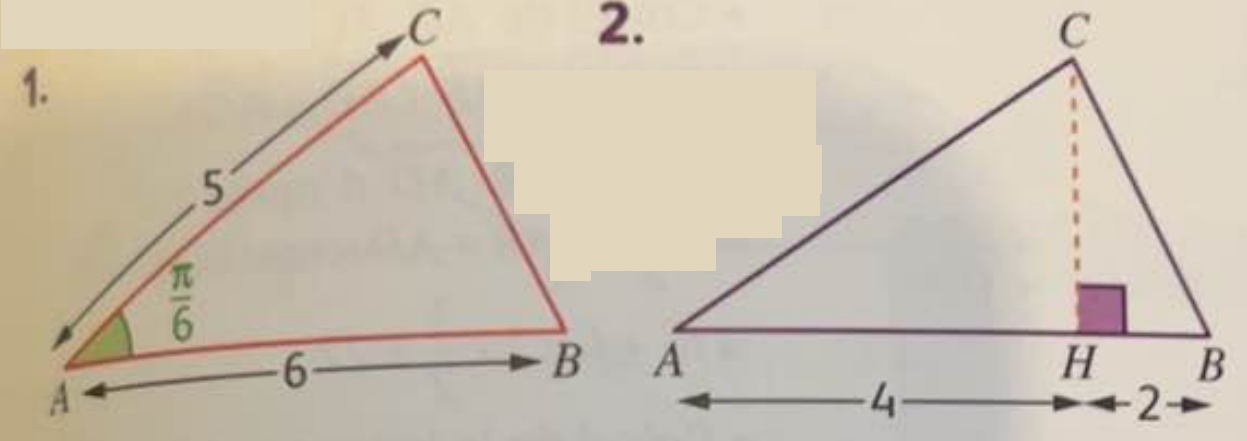
\includegraphics[scale=0.3]{1.04.02-Img01}
\end{center}

\exercice{} 
$A B D$ et $B C D$ sont deux triangles équilatéraux de côté 6. Calculer les produits scalaires suivants.
\begin{multicols}{2}
	\begin{enumMet}
		\begin{multicols}{2}
		\item $\vv{CD} \cdot \vv{CB}$ 
		\item $\vv{DA} \cdot \vv{DC}$
		\item $\vv{D B} \cdot \vv{C B}$
		\item $\vv{DB} \cdot \vv{AC}$
		\item $\vv{A B} \cdot \vv{C D}$
		\item $\vv{CA} \cdot \vv{BC}$
		\end{multicols}
	\end{enumMet}
	\columnbreak
	\begin{center}
		\newrgbcolor{ududff}{0.30196078431372547 0.30196078431372547 1.}
		\newrgbcolor{qqzzqq}{0. 0.6 0.}
		\psset{xunit=0.42cm,yunit=0.42cm,algebraic=true,dimen=middle,dotstyle=o,dotsize=5pt 0,linewidth=2.pt,arrowsize=3pt 2,arrowinset=0.25}
		\begin{pspicture*}(0,0.5)(9.5,5.9)
			\pspolygon[linewidth=1.7pt,linecolor=qqzzqq](5.,5.)(5.,1.)(8.464101615137755,3.)
			\pspolygon[linewidth=1.7pt,linecolor=qqzzqq](5.,5.)(1.5358983848622443,3.)(5.,1.)
			\begin{scriptsize}
				\rput[bl](5.,5.2){\large{$D$}}
				\rput[bl](5.,0.52){\large{$B$}}
				\rput[bl](8.6,2.95){\large{$C$}}
				\rput[bl](1.,2.95){\large{$A$}}
			\end{scriptsize}
		\end{pspicture*}
	\end{center}
\end{multicols}


\exercice{}
Dans chaque cas, calculer $\vv{A B} \cdot \vv{A C}$.
\begin{center}
	\newrgbcolor{ududff}{0.30196078431372547 0.30196078431372547 1.}
	\newrgbcolor{qqwuqq}{0. 0.39215686274509803 0.}
	\psset{xunit=0.8cm,yunit=0.8cm,algebraic=true,dimen=middle,dotstyle=o,dotsize=5pt 0,linewidth=2.pt,arrowsize=3pt 2,arrowinset=0.25}
	\begin{pspicture*}(4,7.5)(17.5,15)
%		\multips(0,2)(0,1.0){18}{\psline[linestyle=dashed,linecap=1,dash=1.5pt 1.5pt,linewidth=0.4pt,linecolor=lightgray]{c-c}(0.98,0)(26.94,0)}
%		\multips(0,0)(1.0,0){26}{\psline[linestyle=dashed,linecap=1,dash=1.5pt 1.5pt,linewidth=0.4pt,linecolor=lightgray]{c-c}(0,2.36)(0,20.02)}
%		\psaxes[labelFontSize=\scriptstyle,xAxis=true,yAxis=true,Dx=1.,Dy=1.,ticksize=-2pt 0,subticks=2]{->}(0,0)(0.98,2.36)(26.94,20.02)
		\pspolygon[linewidth=1.7pt,linecolor=qqwuqq,fillcolor=green,fillstyle=solid,opacity=0.1](13.42426406871193,12.)(13.42426406871193,12.42426406871193)(13.,12.42426406871193)(13.,12.)
		\pspolygon[linewidth=1.7pt,linecolor=qqwuqq,fillcolor=green,fillstyle=solid,opacity=0.1](4.924264068711929,8.)(4.924264068711929,8.42426406871193)(4.5,8.42426406871193)(4.5,8.)
		\psline[linewidth=1.7pt](9.,12.)(5.,12.)
		\psline[linewidth=1.7pt](5.,12.)(6.5,14.6)
		\psline[linewidth=1.7pt](6.5,14.6)(9.,12.)
		\psline[linewidth=1.7pt](11.,12.)(13.,14.4)
		\psline[linewidth=1.7pt,linestyle=dashed](13.,14.4)(13.,12.)
		\psline[linewidth=1.7pt](13.,12.)(11.,12.)
		\psline[linewidth=1.7pt](13.,12.)(16.,12.)
		\psline[linewidth=1.7pt](16.,12.)(13.,14.4)
		\pscustom[linewidth=1.7pt,linecolor=qqwuqq,fillcolor=green,fillstyle=solid,opacity=0.1]{
			\parametricplot{0.0}{1.047518004662921}{0.6*cos(t)+5.|0.6*sin(t)+12.}
			\lineto(5.,12.)\closepath}
		\psline[linewidth=1.7pt,linestyle=dashed](4.5,8.)(6.,8.)
		\psline[linewidth=1.7pt](6.,8.)(10.,8.)
		\psline[linewidth=1.7pt](10.,8.)(4.5,10.36)
		\psline[linewidth=1.7pt](4.5,10.36)(6.,8.)
		\psline[linewidth=1.7pt,linestyle=dashed](4.5,10.36)(4.5,8.)
		\psline[linewidth=1.7pt](17.,8.)(12.,11.)
		\psline[linewidth=1.7pt](12.,11.)(13.,9.)
		\psline[linewidth=1.7pt](13.,9.)(17.,8.)
		\pscustom[linewidth=1.7pt,linecolor=qqwuqq,fillcolor=green,fillstyle=solid,opacity=0.1]{
			\parametricplot{-0.24497866312686414}{2.0344439357957027}{0.6*cos(t)+13.|0.6*sin(t)+9.}
			\lineto(13.,9.)\closepath}
		\rput[tl](4,14.8){$\fbox{\Large{1}}$}
		\rput[tl](10.5,14.8){$\fbox{\Large{2}}$}
		\rput[tl](8.,11){$\fbox{\Large{3}}$}
		\rput[tl](15,11){$\fbox{\Large{4}}$}
		%1ère figure
		\rput[tl](5.4,13.84){\Large{3}}
		\rput[tl](6.8,12.6){\Large{4}}
		\rput[bl](5.64,12.2){\Large{\qqwuqq{$60\degree$}}}
		\rput[bl](4.54,12.12){\Large{$A$}}
		\rput[bl](9.08,12.2){\Large{$B$}}
		\rput[bl](6.6,14.5){\Large{$C$}}
		%2ème figure
		\rput[tl](11.8,12.6){\Large{2}}
		\rput[tl](14.54,12.6){\Large{3,5}}
		\rput[bl](10.66,12.2){\Large{$A$}}
		\rput[bl](12.4,12.1){\Large{$H$}}
		\rput[bl](16.08,12.2){\Large{$B$}}
		\rput[bl](13.08,14.4){\Large{$C$}}
		%3ème figure
		\rput[tl](5.5,9.42){\Large{4}}
		\rput[tl](8.02,7.9){\Large{7}}
		\rput[tl](5.18,7.9){\Large{3}}
		\rput[bl](6.08,8.2){\Large{$A$}}
		\rput[bl](10.08,8.2){\Large{$B$}}
		\rput[bl](4.58,10.56){\Large{$C$}}
		\rput[bl](3.9,8.){\Large{$H$}}
		%4ème figure
		\rput[tl](11.62,10.1){\Large{2}}
		\rput[tl](15.18,8.2){\Large{3}}
		\rput[bl](13.,8.3){\Large{$A$}}
		\rput[bl](17.08,8.2){\Large{$B$}}
		\rput[bl](12.,11.){\Large{$C$}}
		\rput[bl](12.1,8.4){\Large{\qqwuqq{$\frac{3\pi}{4}$}}}
		
		
		
		
	\end{pspicture*}
	%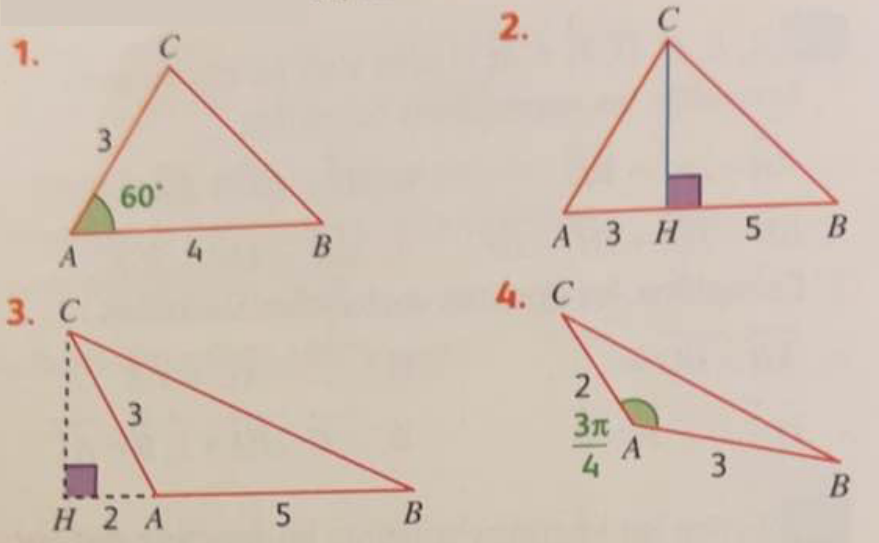
\includegraphics[scale=0.4]{1.04.02-Img03}
\end{center}

\exercice{}
\begin{enumMet}
	\item Pour chaque figure ci-dessous, calculer :
	\begin{enumMet}
		\begin{multicols}{2}
			\item $\|\vv{u}\|$ et $\|\vv{v}\|$ ;
			\item $\vv{u} \cdot \vv{v}$.
		\end{multicols}
	\end{enumMet}
	\item En déduire la valeur de l'angle géométrique $\alpha$.
\end{enumMet}
\begin{center}
	\newrgbcolor{xfqqff}{0.4980392156862745 0. 1.}
	\newrgbcolor{ffxfqq}{1. 0.4980392156862745 0.}
	\newrgbcolor{qqwuqq}{0. 0.39215686274509803 0.}
	\psset{xunit=0.6cm,yunit=0.6cm,algebraic=true,dimen=middle,dotstyle=o,dotsize=5pt 0,linewidth=2.pt,arrowsize=3pt 2,arrowinset=0.25}
	\begin{pspicture*}(1,-0.1)(19,6.1)
		\multips(0,-2)(0,1.0){18}{\psline[linewidth=0.4pt,linecolor=gray]{c-c}(-0.34,0)(25.84,0)}
		\multips(0,0)(1.0,0){27}{\psline[linewidth=0.4pt,linecolor=gray]{c-c}(0,-2.02)(0,15.96)}
		\psline[linewidth=1.7pt,linecolor=xfqqff]{->}(2.,2.)(6.,2.)
		\psline[linewidth=1.7pt,linecolor=ffxfqq]{->}(2.,2.)(5.,5.)
		\psline[linewidth=1.7pt,linecolor=xfqqff]{->}(8.,2.)(10.,0.)
		\psline[linewidth=1.7pt,linecolor=ffxfqq]{->}(8.,2.)(8.,6.)
		\psline[linewidth=1.7pt,linecolor=xfqqff]{->}(13.,3.)(12.,1.)
		\psline[linewidth=1.7pt,linecolor=ffxfqq]{->}(13.,3.)(10.,3.)
		\psline[linewidth=1.7pt,linecolor=xfqqff]{->}(16.,1.)(18.,3.)
		\psline[linewidth=1.7pt,linecolor=ffxfqq]{->}(16.,1.)(15.,4.)
		\pscustom[linewidth=1.7pt,linecolor=qqwuqq,fillcolor=green,fillstyle=solid,opacity=0.1]{
			\parametricplot{0.0}{0.7853981633974483}{0.6*cos(t)+2.|0.6*sin(t)+2.}
			\lineto(2.,2.)\closepath}
		\pscustom[linewidth=1.7pt,linecolor=qqwuqq,fillcolor=green,fillstyle=solid,opacity=0.1]{
			\parametricplot{-0.7853981633974483}{1.5707963267948966}{0.6*cos(t)+8.|0.6*sin(t)+2.}
			\lineto(8.,2.)\closepath}
		\pscustom[linewidth=1.7pt,linecolor=qqwuqq,fillcolor=green,fillstyle=solid,opacity=0.1]{
			\parametricplot{3.141592653589793}{4.2487413713838835}{0.6*cos(t)+13.|0.6*sin(t)+3.}
			\lineto(13.,3.)\closepath}
		\pscustom[linewidth=1.7pt,linecolor=qqwuqq,fillcolor=green,fillstyle=solid,opacity=0.1]{
			\parametricplot{0.7853981633974483}{1.8925468811915387}{0.6*cos(t)+16.|0.6*sin(t)+1.}
			\lineto(16.,1.)\closepath}
		\rput[tl](2.1,5.9){$\fbox{\Large{1}}$}
		\rput[tl](9.2,5.9){$\fbox{\Large{2}}$}
		\rput[tl](11.,5.9){$\fbox{\Large{3}}$}
		\rput[tl](16.,5.9){$\fbox{\Large{4}}$}
		\begin{scriptsize}
			\rput[bl](3.98,2.1){\Large{\xfqqff{$\vv{u}$}}}
			\rput[bl](3.,3.58){\Large{\ffxfqq{$\vv{v}$}}}
			\rput[bl](9.06,1.08){\Large{\xfqqff{$\vv{u}$}}}
			\rput[bl](8.2,4.){\Large{\ffxfqq{$\vv{v}$}}}
			\rput[bl](12.56,1.7){\Large{\xfqqff{$\vv{u}$}}}
			\rput[bl](11.48,3.2){\Large{\ffxfqq{$\vv{v}$}}}
			\rput[bl](16.92,1.2){\Large{\xfqqff{$\vv{u}$}}}
			\rput[bl](15.4,2.48){\Large{\ffxfqq{$\vv{v}$}}}
			\rput[bl](2.68,2.16){\Large{\qqwuqq{$\alpha$}}}
			\rput[bl](8.82,2.){\Large{\qqwuqq{$\alpha$}}}
			\rput[bl](11.9,2.54){\Large{\qqwuqq{$\alpha$}}}
			\rput[bl](15.9,1.76){\Large{\qqwuqq{$\alpha$}}}
		\end{scriptsize}
	\end{pspicture*}
	%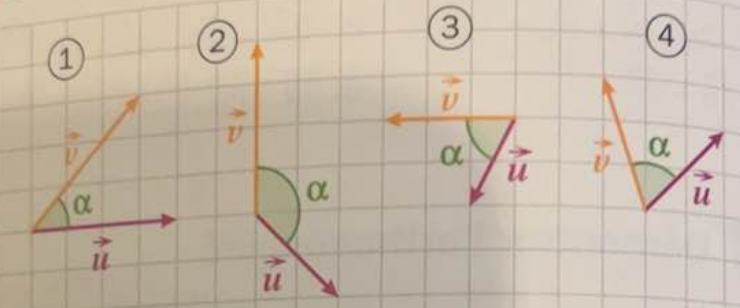
\includegraphics[scale=0.5]{1.04.02-Img02}
\end{center}

\newpage

\exercice{}
calculer $\vv{u} \cdot \vv{v}$ dans chaque cas.
\begin{multicols}{3}
	\begin{enumMet}
		\item $\vv{u}\left(\begin{array}{c}2 \\ -1\end{array}\right)$ et $\vv{v}\left(\begin{array}{l}4 \\ 5\end{array}\right)$.
		\item $\vv{u}\left(\begin{array}{c}\dfrac{1}{2} \\ -3\end{array}\right)$ et $\vv{v}\left(\begin{array}{c}\dfrac{1}{4} \\ \dfrac{1}{3}\end{array}\right)$.
		\item $\Coord{u}{3}{2}$ et $\Coord{v}{3}{1}$.
	\end{enumMet}
\end{multicols}


\exercice{}
$\vv{u}\left(\begin{array}{c}1 \\ -3\end{array}\right)$ et $\vv{v}\left(\begin{array}{c}1 \\ -1\end{array}\right)$ sont deux vecteurs du plan. calculer les produits scalaires suivants.
\begin{multicols}{4}
\begin{enumMet}
	\item $\vv{u} \cdot \vv{v}$
	\item $\vv{u} \cdot(-4 \vv{v})$
	\item $-\vv{u} \cdot(2 \vv{v})$
	\item $(\vv{u}+\vv{v}) \cdot(\vv{u}-\vv{v})$
\end{enumMet}
\end{multicols}

\exercice{}
$A(-2 ; 5), B(4 ; 3)$ et $C(1 ;-6)$ sont trois points du plan.
\begin{enumMet}
	\item Determiner les coordonnées des vecteurs $\vv{B A}$ et $\vv{B C}$.
	\item Calculer $\vv{B A} \cdot \vv{B C}$.
	\item En déduire la nature du triangle $A B C$.
\end{enumMet}

\exercice{}
On donne $\mathrm{A}(2 ;-1), \mathrm{B}(0 ; 1)$ et $\mathrm{C}(1 ;-2)$.
\begin{enumMet}
	\item Calculer $A B$ et $A C$.
	\item Calculer $\vv{AB} \cdot \vv{AC}$.
	\item Calculer une mesure de l'angle $(\vv{AB}, \vv{AC})$.
\end{enumMet}

\exercice{}
Dans un repère orthonormé, on considère les points $A(0 ; 4), B(6 ; 3)$ et $C(-4 ;-2)$.\\
Calculer $\vv{A B} \cdot \vv{A C}$ de deux façons différentes pour déterminer une mesure en degré de l'angle $\widehat{B A C}$.

\exercice{}
Dans un repère orthonormé, on donne les points : $M(2;-2)$, $N(-3;1)$ et $P(1;2)$
\begin{enumMet}
	\item Calculer $\vv{M N} \cdot \vv{M P}$.
	\item En déduire une valeur exacte de l'angle $\widehat{P M N}$.
\end{enumMet}

\exercice{}
Dans un repère orthonormé, on donne les points $A(1 ; 1), B\left(\dfrac{14}{5} ; \dfrac{17}{5}\right)$ et $C(5 ; 1)$.
\begin{enumMet}
	\item Calculer les produits scalaires suivants.
	\begin{enumMet}
		\begin{multicols}{3}
		\item $\vv{A B} \cdot \vv{A C}$
		\item $\vv{C A} \cdot \vv{C B}$
		\item $\vv{B A} \cdot \vv{B C}$
		\end{multicols}
	\end{enumMet}
	\item Le triangle $A B C$ est-il rectangle ?
\end{enumMet}

\exercice{}
\begin{multicols}{2}
	On considere les vecteurs $\vv{u}$ et $\vv{v}$ représentés ci-contre.\\
	On donne $\|\vv{u}\|=2,\|\vv{v}\|=3$ et $\theta=\dfrac{2 \pi}{3}$. Calculer les eléments suivants.
	\begin{enumMet}
		\item $\vv{u} \cdot \vv{v}$
		\item $3 \vv{v} \cdot(\vv{u}-2 \vv{v})$
		\item $\|\vv{u}+\vv{v}\|^2$
		%\item $\|2 \vv{u}-\vv{v}\|$
	\end{enumMet}
	\columnbreak
	\begin{center}
		\newrgbcolor{qqwuqq}{0. 0.39215686274509803 0.}
		\psset{xunit=1.2cm,yunit=1.2cm,algebraic=true,dimen=middle,dotstyle=o,dotsize=5pt 0,linewidth=2.pt,arrowsize=3pt 2,arrowinset=0.25}
		\begin{pspicture*}(0.5,1.7)(4.2,5.2)
			\psline[linewidth=1.7pt]{->}(2.,2.)(4.,2.)
			\psline[linewidth=1.7pt]{->}(2.,2.)(1.,5.)
			\pscustom[linewidth=1.7pt,linecolor=qqwuqq,fillcolor=green,fillstyle=solid,opacity=0.1]{
				\parametricplot{0.0}{1.892546881191539}{0.6*cos(t)+2.|0.6*sin(t)+2.}
				\lineto(2.,2.)\closepath}
			%\begin{scriptsize}
				\rput[bl](3.,2.1){\Large{$\vv{u}$}}
				\rput[bl](1.,3.16){\Large{$\vv{v}$}}
				\rput[bl](2.54,2.48){\Large{\qqwuqq{$\theta$}}}
			%\end{scriptsize}
		\end{pspicture*}
	\end{center}
\end{multicols}

\end{document}

